% -*- root: main.tex -*-

\chapter{Loose ends}

---

\todo[inline]{I'd like to spend a couple of days talking about ways the picture in this class can be extended, finally, some actually unanswered questions that naturally arise.  The following two section titles are totally made up and probably won't last.}

\section{\texorpdfstring{$E_\infty$}{Eoo} geometry}

\Cref{OrdinaryHomologyInUpperHalfPlaneEx} is an inspiration for considering $\tmf$ as well.



\subsection*{The modularity of the $M\String$ orientation}

$E_\infty$ orientations by $M\String$

$\tmf$, $\TMF$, and $\Tmf$ in terms of $\moduli{ell}$

Thom spectra and $\infty$--categories

The Bousfield--Kuhn functor and the Rezk logarithm

% free $E_\infty$--orientations off of $MU$



\section{Rational phenomena: character theory for Lubin--Tate spectra}

There's a sufficient amount of reliance on character theory in Matt's thesis that we should talk about it.  You should write that action and then backtrack here to see what you need for it.

See Morava's \textit{Local fields} paper

\begin{remark}
Theorem 2.6 of Greenlees--Strickland for a nice transchromatic perspective.  See also work of Stapleton and Schlank--Stapleton, of course.\todo{Flesh this out.}
\end{remark}


------

\begin{theorem}\citeme{Theorem A}
Let $E$ be any complex-oriented cohomology theory.  Take $G$ to be a finite group and let $\CatOf{Ab}_G$ be the full subcategory of the orbit category of $G$ built out of abelian subgroups of $G$.  Finally, let $X$ be a finite $G$--CW complex.  Then, each of the natural maps \[E^*(EG \times_G X) \to \lim_{A \in \CatOf{Ab}_G} E^*(EG \times_A X) \to \int_{A \in \CatOf{Ab}_G} E^*(BA \times X^A)\] becomes an isomorphism after inverting the order of $G$.  In particular, there is an isomorphism \[\frac{1}{|G|} E^* BG \to \lim_{A \in \CatOf{Ab}_G} \frac{1}{|G|} E^* BA. \qed\]
\end{theorem}

This is an analogue of Artin's theorem:
\begin{theorem}
There is an isomorphism \[\frac{1}{|G|} R(G) \to \lim_{C \in \CatOf{Cyclic}_G} \frac{1}{|G|} R(C). \qed\]
\end{theorem}


------

HKR intro material connecting Theorem A to character theory:

Recall that classical characters for finite groups are defined in the following situation: take $L = \Q^{\mathrm{ab}}$ to be the smallest characteristic $0$ field containing all roots of unity, and for a finite group $G$ let $Cl(G; L)$ be the ring of class functions on $G$ with values in $L$.  The units in the profinite integers $\widehat{\Z}$ act on $L$ as the Galois group over $\Q$, and since $G = \CatOf{Groups}(\widehat{\Z}, G)$ they also act naturally on $G$.  Together, this gives a conjugation action on $Cl(G; L)$: for $\phi \in \widehat{\Z}$, $g \in G$, and $\chi \in Cl(G; L)$, one sets \[(\phi \cdot \chi)(g) = \phi(\chi(\phi^{-1}(g))).\]  The character map is a ring homomorphism \[\chi: R(G) \to Cl(G; L)^{\widehat{\Z}},\] and this induces isomorphisms \[\chi: L \otimes R(G) \xrightarrow{\simeq} Cl(G; L)\] and even \[\chi: \Q \otimes R(G) \xrightarrow{\simeq} Cl(G; L)^{\widehat{\Z}}.\]

Now take $E = E_\Gamma$ to be a Morava $E$--theory of finite height $d = \height(\Gamma)$.  Take $E^*(B\Z_p^d)$ to be topologized by $B(\Z/p^j)^d$.  A character $\alpha: \Z_p^d \to S^1$ will induce a map $\alpha^*: E^* \CP^\infty \to E^* B\Z_p^d$.  We define $L(E^*) = S^{-1} E^*(B\Z_p^d)$, where $S$ is the set of images of a coordinate on $\CP^\infty_E$ under $\alpha^*$ for nonzero characters $\alpha$.  Note that this ring inherits an $\operatorname{Aut}(\Z_p^d)$ action by $E^*$--algebra maps.

The analogue of $Cl(G; L)$ will be $Cl_{d,p}(G; L(E^*))$, defined to be the ring of functions $\chi: G_{d, p} \to L(E^*)$ stable under $G$--orbits.  Noting that \[G_{d,p} = \operatorname{Hom}(\Z_p^d, G),\] one sees that $\operatorname{Aut}(\Z_p^d)$ acts on $G_{d,p}$ and thus on $Cl_{d,p}(G; L(E^*))$ as a ring of $E^*$--algebra maps: given $\phi \in \operatorname{Aut}(\Z_p^d)$, $\alpha \in G_{d,p}$, and $\chi \in Cl_{d,p}(G; L(E^*))$ one lets \[(\phi \cdot \chi)(\alpha) = \phi(\chi(\phi^{-1}(\alpha))).\]

Now we introduce a finite $G$--CW complex $X$.  Let \[\operatorname{Fix}_{d, p}(G, X) = \coprod_{\alpha \in \operatorname{Hom}(\Z_p^d, G)} X^{\operatorname{im} \alpha}.\]  This space has commuting actions of $G$ and $\operatorname{Aut}(\Z_p^d)$.  We set \[Cl_{d, p}(G, X; L(E^*)) = L(E^*) \otimes_{E^*} E^*(\operatorname{Fix}_{d,p}(G, X))^G,\] which is again an $E^*$--algebra acted on by $\operatorname{Aut}(Z_p^d)$.  We define the character map ``componentwise'': a homomorphism $\alpha \in \operatorname{Hom}(\Z_p^d, G)$ induces \[E^*(EG \times_G X) \to E^*(B\Z_p^d) \otimes_{E^*} E^*(X^{\operatorname{im} \alpha}) \to L(E^*) \otimes_{E^*} E^*(X^{\operatorname{im} \alpha}).\]  Taking the direct sum over $\alpha$, this assembles into a map \[\chi_{d,p}^G: E^*(EG \times_G X) \to Cl_{d,p}(G, X; L(E^*))^{\operatorname{Aut}(Z_p^d)}.\]
\todo{Nat taught you how to say all these things with $p$--adic tori, which was \emph{much} clearer.}
\begin{theorem}\citeme{Theorem C}
The invariant ring is $L(E^*)^{\operatorname{Aut}(\Z_p^d)} = p^{-1} E^*$, and $L(E^*)$ is faithfully flat over $p^{-1} E^*$.\todo{Checking this invariant ring claim is easiest done by comparing the functors the two things corepresent.}  The character map $\chi_{d,p}^G$ induces isomorphisms
\begin{align*}
\chi_{d,p}^G \co L(E^*) \otimes_{E^*} E^*(EG \times_G X) & \xrightarrow{\simeq} Cl_{d,p}(G, X; L(E^*)), \\
\chi_{d,p}^G \co p^{-1} E^*(EG \times_G X) & \xrightarrow{\simeq} Cl_{d,p}(G, X; L(E^*))^{\operatorname{Aut}(\Z_p^d)}.
\end{align*}
In particular, when $X = *$, there are isomorphisms
\begin{align*}
\chi_{d,p}^G \co L(E^*) \otimes_{E^*} E^*(BG) & \xrightarrow{\simeq} Cl_{d,p}(G; L(E^*)), \\
\chi_{d,p}^G \co p^{-1} E^*(BG) & \xrightarrow{\simeq} Cl_{d,p}(G; L(E^*))^{\operatorname{Aut}(\Z_p^d)}. \qed
\end{align*}
\end{theorem}

------

Jack gives an interpretation of this in terms of formal $\sheaf{O}_L$--modules.

------

I also have this summary of Nat's of the classical case:

It's not easy to decipher if you weren't there for the conversation, but here's my take on it. First, the map we wrote down today was the non-equivariant chern character: it mapped non-equivariant $KU \otimes \Q$ to non-equivariant $H\Q$, periodified. The first line on Nat's board points out that if you use this map on Borel-equivariant cohomology, you get nothing interesting: $K^0(BG)$ is interesting, but $H\Q^*(BG) = H\Q^*(*)$ collapses for finite $G$. So, you have to do something more impressive than just directly marry these two constructions to get something interesting.

That bottom row is Nat's suggestion of what ``more interesting'' could mean. (Not really his, of course, but I don't know who did this first. Chern, I suppose.) For an integer $n$, there's an evaluation map of (forgive me) topological stacks \[* \mmod (\Z/n) \times \operatorname{Hom}(* \mmod (\Z/n), * \mmod G) \xrightarrow{\mathrm{ev}} * \mmod G\] which upon applying a global-equivariant theory like $K_G$ gives \[K_{\Z/n}(*) \otimes K_G(\coprod_{\text{conjugacy classes of $g$ in $G$}} *) \xleftarrow{ev^*} K_G(*).\]

Now, apply the genuine $G$-equivariant Chern character to the $K_G$ factor to get \[K_{\Z/n}(*) \otimes H\Q_G(\coprod *) \from K_{\Z/n}(*) \otimes K_G(\coprod *),\] where the coproduct is again taken over conjugacy classes in G. Now, compute $K_{\Z/n}(*) = R(\Z/n) = \Z[x] / (x^n - 1)$, and insert this calculation to get \[K_{\Z/n}(*) \otimes H\Q_G(\coprod *) = \Q(\zeta_n) \otimes (\bigoplus_{\text{conjugacy classes}} \Q),\] where $\zeta_n$ is an $n${\th} root of unity.  As $n$ grows large, this selects sort of the part of the complex numbers $\C$ that the character theory of finite groups cares about, and so following all the composites we've built a map \[K_G(*) \to \C \otimes (\bigoplus_{\text{conjugacy classes}} \C).\]  The claim, finally, is that this map sends a $G$-representation (thought of as a point in $K_G(*)$) to its class function decomposition.


-----




\section{The period map}\label{ThePeriodMapSection}

\todo{pp.\ 42-43 of FPFP has some easy-to-state results about this collected.}
\todo{Kohlhaase~\cite{Kohlhaase} references Yu~\cite{Yu} for having closed formulas generalizing the Hopkins--Gross example section.}

Describe Dieudonn\'e crystals and the Tapis de Cartier.

Show how Dieudonn\'e crystals are used to give formulas for the action of the stabilizer group~\cite{DevinatzHopkins}.

Give a sketch explanation of the Gross--Hopkins period map~\cite{Weinstein}.

Draw the picture of the period map at $n = 2$, $p = 2$.  The main reference for this, except for the literal picture, is~\cite[Appendix 25]{HopkinsGrossEquivVBs}.
\begin{itemize}
\item The center of the $\Z_{p^2}$--points of Lubin--Tate space corresponds to the canonical lift, which is the formal group that further acquires an $\mathcal O_A$--module structure.  It has $\pi$--series $[\pi](x) = \pi x + x^{q^2}$.
\item There are three nontrivial points in $\G[2]$: $\alpha$, $\beta$, and $\alpha + \beta$.  Quotienting by them gives three points at order $1/(q+1)$, the first bunch of ``quasicanonical lifts'', which have partial formal $\mathcal O_A$--module structures.
\item At each quasicanonical point, you also also form three quotients: two of them make the situation ``worse'', and one of them makes the situation ``better''.  This has to do with the identification $\G / \G[2] \cong \G$.
\item Computing these orders has to do with the Newton polygon associated to the $\pi$--series.
\item The canonical Frobenius $F_{can} = \left[ \begin{array}{cc} 0 & p \\ 1 & 0 \end{array} \right]$ first flips the two coordinates (and scales one by $p$), then flips them back (and scales the other by $p$), and after two flips scaling everything by $p$ scales back down by homogeneous coordinates.
\item Out to order $1/q$, $\pi_{GH}$ is injective.
\item The group $\F_4^\times$ should act by rotation on $\mathbb P^1$.
\item The map $\pi_{GH}$ sends the canonical lift to $0 = [1:0]$, sends the first order quasicanonical points to $\infty = [0:1]$, and alternates from there.  The three branches of ``directions to quotient'' carve $\mathbb P^1$ up into three lobes.  This is because $\pi_{GH}$ is equivariant for \emph{isogenies}, and quotienting by one of these order $2$ subgroups is a lift of the Frobenius isogeny on the residue formal group.
\item These quasicanonical points are the ones with nontrivial stabilizers under the action by the Morava stabilizer group --- all the other points belong to free orbits.  (The canonical lift has the largest stabilizer of all.)
\end{itemize}

\begin{figure}
\begin{center}

\pgfdeclareradialshading{myshading}{\pgfpointorigin}
{
  color(0cm)=(pgftransparent!100);
  color(2cm)=(pgftransparent!100);
  color(2.5cm)=(pgftransparent!0);
  color(3cm)=(pgftransparent!0)
}
\pgfdeclarefading{fading3}{\pgfuseshading{myshading}}

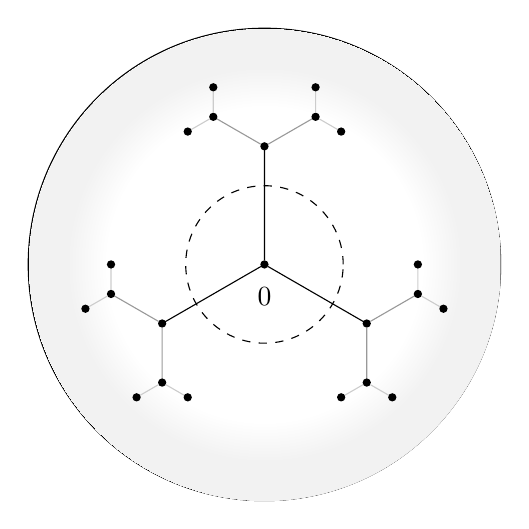
\begin{tikzpicture}[baseline=(current bounding box.center)]
% thanks to Tomasz M. Trzeciak
% based off of http://www.latex-community.org/viewtopic.php?f=4&t=2111

\draw (0,0) circle (3);

\begin{scope}
\pgfsetfading{fading3}{\pgftransformshift{\pgfpoint{0cm}{0cm}}}
\filldraw[black!5] (0,0) circle (3);
\end{scope}

\draw[dashed] (0,0) circle (1);
\coordinate[style={inner sep=0pt, outer sep=0pt, minimum size=3pt, fill=black, circle}] (O) at (0,0);
\node[below=5pt] at (O) {$0$};

\draw (O) -- +( 90:1.5) coordinate[style={inner sep=0pt, outer sep=0pt, minimum size=3pt, fill=black, circle}] (Q1)
      (O) -- +(210:1.5) coordinate[style={inner sep=0pt,outer sep=0pt,minimum size=3pt, fill=black,circle}] (Q2)
      (O) -- +(330:1.5) coordinate[style={inner sep=0pt,outer sep=0pt,minimum size=3pt, fill=black,circle}] (Q3);

\draw[black!40] (Q1) -- +(120-90:0.75) coordinate[style={inner sep=0pt, outer sep=0pt, minimum size=3pt, fill=black, circle}] (Q12)
      (Q1) -- +(240-90:0.75) coordinate[style={inner sep=0pt, outer sep=0pt, minimum size=3pt, fill=black, circle}] (Q13)
      (Q2) -- +(120-330:0.75) coordinate[style={inner sep=0pt, outer sep=0pt, minimum size=3pt, fill=black, circle}] (Q21)
      (Q2) -- +(240-330:0.75) coordinate[style={inner sep=0pt, outer sep=0pt, minimum size=3pt, fill=black, circle}] (Q23)
      (Q3) -- +(120-210:0.75) coordinate[style={inner sep=0pt, outer sep=0pt, minimum size=3pt, fill=black, circle}] (Q31)
      (Q3) -- +(240-210:0.75) coordinate[style={inner sep=0pt, outer sep=0pt, minimum size=3pt, fill=black, circle}] (Q32);

\draw[black!20] (Q12) -- +(90:0.375) coordinate[style={inner sep=0pt, outer sep=0pt, minimum size=3pt, fill=black, circle}] (Q121)
      (Q12) -- +(330:0.375) coordinate[style={inner sep=0pt, outer sep=0pt, minimum size=3pt, fill=black, circle}] (Q123)
      (Q13) -- +(90:0.375) coordinate[style={inner sep=0pt, outer sep=0pt, minimum size=3pt, fill=black, circle}] (Q131)
      (Q13) -- +(210:0.375) coordinate[style={inner sep=0pt, outer sep=0pt, minimum size=3pt, fill=black, circle}] (Q132)
      (Q21) -- +(90:0.375) coordinate[style={inner sep=0pt, outer sep=0pt, minimum size=3pt, fill=black, circle}] (Q212)
      (Q21) -- +(210:0.375) coordinate[style={inner sep=0pt, outer sep=0pt, minimum size=3pt, fill=black, circle}] (Q213)
      (Q23) -- +(210:0.375) coordinate[style={inner sep=0pt, outer sep=0pt, minimum size=3pt, fill=black, circle}] (Q231)
      (Q23) -- +(330:0.375) coordinate[style={inner sep=0pt, outer sep=0pt, minimum size=3pt, fill=black, circle}] (Q232)
      (Q31) -- +(210:0.375) coordinate[style={inner sep=0pt, outer sep=0pt, minimum size=3pt, fill=black, circle}] (Q312)
      (Q31) -- +(330:0.375) coordinate[style={inner sep=0pt, outer sep=0pt, minimum size=3pt, fill=black, circle}] (Q313)
      (Q32) -- +(90:0.375) coordinate[style={inner sep=0pt, outer sep=0pt, minimum size=3pt, fill=black, circle}] (Q321)
      (Q32) -- +(330:0.375) coordinate[style={inner sep=0pt, outer sep=0pt, minimum size=3pt, fill=black, circle}] (Q323);
\end{tikzpicture}%
%
\quad $\xrightarrow{\pi_{GH}}$ \quad%
%
\begin{tikzpicture}[baseline=(current bounding box.center)]

\newcommand\pgfmathsinandcos[3]{%
  \pgfmathsetmacro#1{sin(#3)}%
  \pgfmathsetmacro#2{cos(#3)}%
}
\newcommand\LongitudePlane[3][current plane]{%
  \pgfmathsinandcos\sinEl\cosEl{#2} % elevation
  \pgfmathsinandcos\sint\cost{#3} % azimuth
  \tikzset{#1/.style={cm={\cost,\sint*\sinEl,0,\cosEl,(0,0)}}}
}
\newcommand\DrawLongitudeCircle[2][1]{
  \LongitudePlane{35}{#2} % first argument is angle of elevation
  \tikzset{current plane/.prefix style={scale=#1}}
   % angle of "visibility"
  \pgfmathsetmacro\angVis{atan(sin(#2)*cos(35)/sin(35))} % these are angle of elevation too
  % this might assume that the angle of elevation is positive
  \draw[current plane] (\angVis:1) arc (\angVis:90:1);
  \draw[current plane,dashed] (\angVis:1) arc (\angVis:-90:1);
}

% the "2.5" magic number is the radius of the sphere 
% the "35" magic number is the angle of elevation of the camera
\pgfmathsetmacro\H{2.5*cos(35)}
\filldraw[ball color=white] (0,0) circle (2.5);
\foreach \t in {-5,-125,-245} { \DrawLongitudeCircle[2.5]{\t} }
\coordinate[style={inner sep=0pt,outer sep=0pt,minimum size=3pt,
    fill=black,circle}] (O) at (0,-\H);
\node[below=16pt] at (O) {$0$};
\coordinate[style={inner sep=0pt,outer sep=0pt,minimum size=3pt,
    fill=black,circle}] (I) at (0,\H);
\node[above=16pt] at (I) {$\infty$};
\end{tikzpicture}
\end{center}

\caption{The period map at $n = 2$, $p = 2$}
\end{figure}

\begin{theorem}\citeme{\cite{HopkinsGrossAnnouncement,StricklandGHDuality}}
\todo{Make sure you get this right.}
The sheaf $\context{E_\Gamma}(\mathbb I_{\Q/\Z})$ is the dualizing sheaf on $(\moduli{fg})^\wedge_\Gamma$. \qed
\end{theorem}





\section{Knowns and unknowns}



\subsection*{Higher orientations}

$\TAF$ and friends\label{TAFDiscussion}

The $\alpha_{1/1}$ argument: Prop 2.3.2 of Hovey's $v_n$--elements of ring spectra

% The HLP calculations

\subsection*{Equivariance}

This is tied up with the theory of power operations in a way I've never really thought about.  Seems complicated.

You should also mention the ``rigidity'' of the elliptic genus, which is about an $S^1$--equivariant version.

\subsection*{Index theorems}

Connections with analysis

The Stolz--Teichner program








-----

Contexts for structured ring spectra

Difficulty in computing $\S_d \actson E_d^*$. (Gross--Hopkins and the period map.)

Barry's $p$--adic measures

Fixed point spectra and e.g. $L_{K(2)} \tmf$.

Blueshift, A--M--S, and the relationship to A--F--G?

Does $E_n$ receive an $E_\infty$ orientation?  Does $BP$?

Remark 12.13 of published $H_\infty$ AHS says their obstruction framework agrees with the $E_\infty$ obstruction framework (if you take everything in sight to have $E_\infty$ structures).  This is almost certainly related to the discussion at the end of Matt's thesis about the $MU$--orientation of $E_d$.\todo{Section 12.4 compares doing $H_\infty$ descent with doing $E_\infty$ descent and shows that they're the same (in the case of interest?).}

Hovey's paper on $v_n$--periodic elements in ring spectra.  He has a nice (and thorough!) exposition on why one should be interested in bordism spectra and their splittings: for instance, a careful analysis of $M\Spin$ will inexorably lead one toward studying $KO$.  It would be nice if studying $M\String$ (and potentially higher analogues) would lead one toward non-completed, non-connective versions of $EO_n$.  Talk about $BoP$, for instance.

Matt's short resolutions of chromatically localized $MU$.






\begin{remark}
It is completely unclear why $MU$ plays such an important mediating role between geometry (i.e., the stable category) and algebra (i.e., sheaves on the moduli of formal groups).  Given a general ring spectrum $R$ and thick prime $\otimes$--ideals $\CatOf C_\alpha$ of perfect $R$--modules, one ask the analogous two questions:
\begin{enumerate}
\item Is it possible to find an $R$--algebra $S$ whose context functor induces a homeomorphism of Balmer spectra $\Spec(\CatOf{Modules}_R^{\perf}) \to \Spec(\CatOf{QCoh}(\context{S/R}))$?
\item Are there complementary localizers $L_\alpha\co \CatOf{Modules}_R \to \CatOf{Modules}_{R,(\alpha)}$?  Can they be presented via Bousfield's framework as homological localizations for auxiliary $S$--algebra spectra $S_\alpha$?  Do the contexts $\context{S_\alpha}$ admit compatible localizers with $\context{S}$?
\end{enumerate}
For $R = \S$, this is the role that the $R$--algebra $S = MU$ and the $S$--algebras $S_d = E(d)$ play.  Finding these spectra feels like striking gold, and it is unclear how to produce analogous spectra in general.
\end{remark}




\begin{remark}
The homotopy of $\widehat L_2 \S$ is also known, by work of Shimomura and collaborators~\cite{Shimomura,ShimomuraYabeM20,ShimomuraYabeL2S} (but see also the reorganization by Behrens~\cite{BehrensRevisited}).  It is \emph{exceedingly} complicated, and it is an open problem to find an expression of it which admits human digestion.  Behrens has pursued a program encoding this problem in terms of modular forms~\cite{BehrensCongruences,BehrensModularDescription,BehrensBuildings}, and Hopkins has proposed a program involving $L$--functions~\cite{StricklandpAdicInterpolation}, motivated by which Hovey and Strickland have shown a kind of continuity result for among the groups~\cite[Section 14]{HoveyStrickland}.
\end{remark}





\begin{remark}
There are also ``finitary'' flavors of chromatic localization available, which are typically less robust but more computable.  They assemble into a diagram:
\begin{center}
\begin{tikzcd}
E \arrow{r} \arrow{d} & L_d^{\fin} E \arrow{r} \arrow{d} & L_d E \arrow{d} \\
L_{X(d)} E \arrow{r} & \widehat L_d^{\fin} E \arrow{r} & \widehat L_d E,
\end{tikzcd}
\end{center}
where $X(d)$ is a finite complex of type exactly $d$, $v$ is a $v_d$--self-map of $X(d)$, $T(d) = X(d)[v^{-1}]$ is the localizing telescope, $\widehat L_d^{\fin}$ is Bousfield localization with respect to $T(d)$ (which can be shown to be independent of choice of $X(d)$ and of $v$), and $L_d^{\fin}$ denotes localization with respect to the class of \emph{finite} $E(d)$--acyclics.  Many things about these functors are known: for instance, $L_{X(d)} L_d = \widehat L_d$, there is a chromatic fracture square relating $L_d^{\fin}$ to $\widehat L_{\le d}^{\fin}$, and $L_d^{\fin} E \simeq L_d E$ if and only if $\widehat L_{\le d}^{\fin} E \simeq \widehat L_{\le d} E$.  One major question about these functors remains open, corresponding the last unsettled nilpotence and periodicity conjecture of Ravenel~\cite[Conjecture 10.5]{RavenelLocalizationWRTPeriodic}: is the map $\widehat L_d^{\fin} E \to \widehat L_d E$ an equivalence?  Multiple proofs and disproofs have been offered, but the literature remains unsettled.
\citeme{Find some proofs and disproofs.}
\end{remark}







\begin{remark}
Writing $M_d$ for the fiber in the sequence $M_d \to L_d \to L_{d-1}$, the filtration spectral sequence associated to the tower in \Cref{ChromaticConvergence} is called the \textit{geometric chromatic spectral sequence}, which has the form $\pi_* M_* \S \Rightarrow \pi_* \S_{(p)}$.  The two forms of filtration data $M_d X$ and $\widehat L_d X$ are actually functorially equivalent to one another:
\begin{align*}
\widehat L_d M_d & \simeq \widehat L_d, &
M_d \widehat L_d & \simeq M_d,
\end{align*}
but they have fairly distinct properties.  For instance, $M_d$ is smashing whereas $\widehat L_d$ is not, $M_d$ is not part of an adjoint pair whereas $\widehat L_d$ is, and the analogue of \Cref{FormulaForKnLocalization} for $M_d$ is ``backwards'':\citeme{I forget who this is due to} \[M_d X \simeq \colim_I \left( M^0(v^I) \sm L_d X \right).\]  The spectrum $M_d X$ also relates to the chromatic fracture square for $X$:
\begin{center}
\begin{tikzcd}
M_d X \arrow{d} \arrow[equal]{r} & M_d X \arrow{d} \\
L_d X \arrow{r} \arrow{d} \arrow[dr, phantom, "\lrcorner", very near start] & \widehat L_d X \arrow{d} \\
L_{d-1} X \arrow{r} & L_{d-1} \widehat L_d X.
\end{tikzcd}
\end{center}
From this, we see that there is a fiber sequence $M_d X \to \widehat L_d X \to L_{d-1} \widehat L_d X$.

The case $d = 1$ gives the prototypical example of the difference between these two presentations of the ``exact height $d$ data'', where the sequence becomes: \[\colim_j (M^0(p^j) \sm L_1 X) \to \lim_j (M_0(p^j) \sm L_1 X) \to \left( \lim_j (M_0(p^j) \sm L_1 X) \right)_{\Q}.\]  If, for instance, $\pi_0 L_1 X = \Z_{(p)}$, then the long exact sequence of homotopy groups associated to this fiber sequence gives
\begin{center}
\begin{tikzcd}
\pi_0 \widehat L_1 X \arrow{r} \arrow[equal]{d} & \pi_0 L_0 \widehat L_1 X \arrow{r} \arrow[equal]{d} & \pi_{-1} M_1 X \arrow[equal]{d} \\
\Z^\wedge_p \arrow{r} & \Q_p \arrow{r} & \Z/p^\infty.
\end{tikzcd}
\end{center}
Coupling this to \Cref{piLK1SExample}, we compute
\begin{align*}
\pi_t M_1 \S^0 & = \begin{cases} \Z/p^\infty & \text{when $t = -1$}, \\ \Z_p / (pk) & \text{when $t = k|v_1| - 1$ and $t = \ne 0$}, \\ \Z/p^\infty & \text{when $t = (0 \cdot |v_1| - 1) - 1 = -2$}, \\ 0 & \text{otherwise}. \end{cases}
\end{align*}
This is a model for what happens generally when passing from $\pi_* \widehat L_d X$ to $\pi_* M_d X$: the $v_j$--torsion--free groups get converted to infinitely $v_j$--divisible groups, with some dimension shifts.\footnote{A height $2$ example of this same phenomenon is visible in Behrens's paper~\cite[Section 7]{BehrensRevisited}.}
\end{remark}





